\Transcb{yellow}{blue}{Search for a diffuse cosmic $\nu$ flux}
\twocolumn
\begin{itemize}
\item Many point sources : diffuse $\nu$ flux
\item[] Expected flux $\sim E^{-2}$
\item[] (Fermi shock acceleration)
\item[] Observed in TeV photons
\item CR primaries : flux $\sim E^{-2.7}$
\item[] $\rightarrow$ Calculate atm. $\nu$ $E$-spectrum
\item $\nu$ det. observe atm. $\nu$ spectrum
\item[] Validate calculated spectrum
\item[$\ast$] {\blue PDF for atm. $\nu$ $E$-spectrum}
\item Very high E : Nearly atm. bkg free
\item[] 0.1 atm. $\nu$ km$^{-3}$ year$^{-1}$ at 1 PeV
\item[] \colorbox{yellow}{VHE events might prove cosmic $\nu$}
\end{itemize}

\newpage 

\begin{center}
{\blue IceCube atmospheric $\nu$ spectrum}\\
{\large [Eur. Phys. J. C75 (2015) 116]}\\
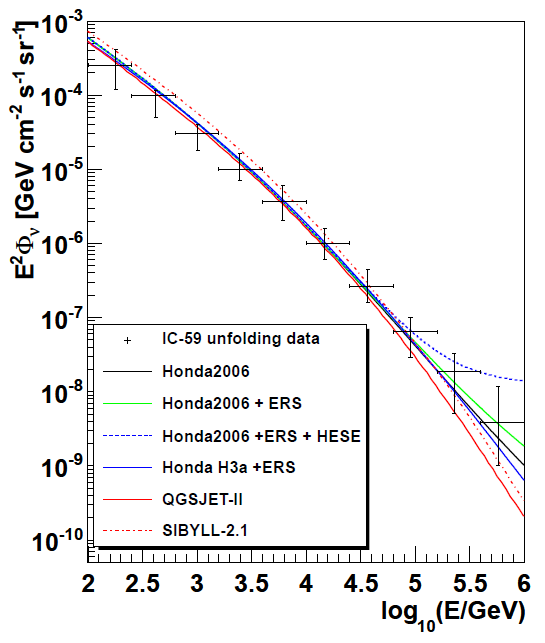
\includegraphics[keepaspectratio,height=14cm]{atm-nu2}
\end{center}

\Tr
\begin{center}
{\blue Tue 09-aug-2011 07:23:18 UTC}\\
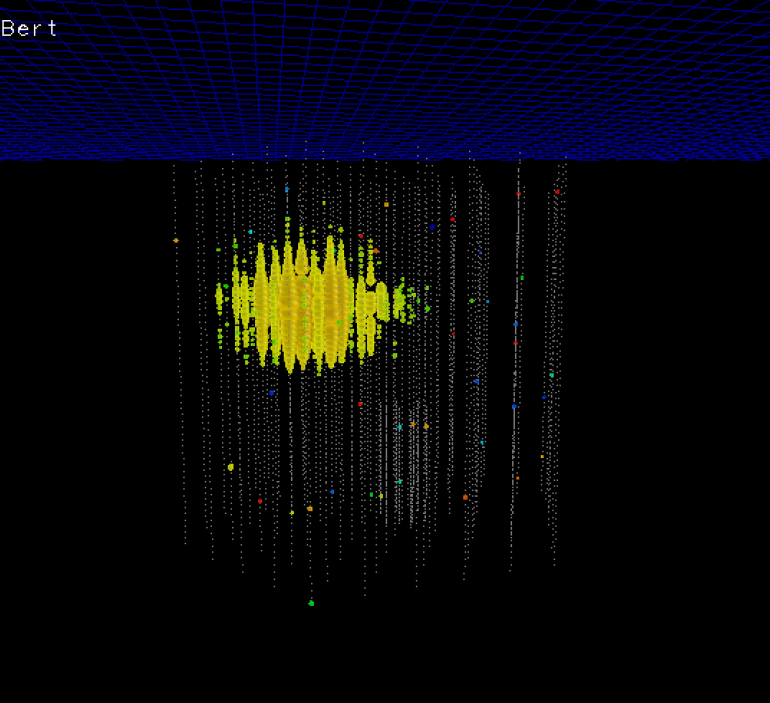
\includegraphics[keepaspectratio,width=13cm]{bert}\\
$1.04 \pm 0.14$ PeV
\end{center}
{\blue Atmospheric $\nu$ background ?}

\newpage

\begin{center}
{\blue Tue 03-jan-2012 03:34:01 UTC}\\
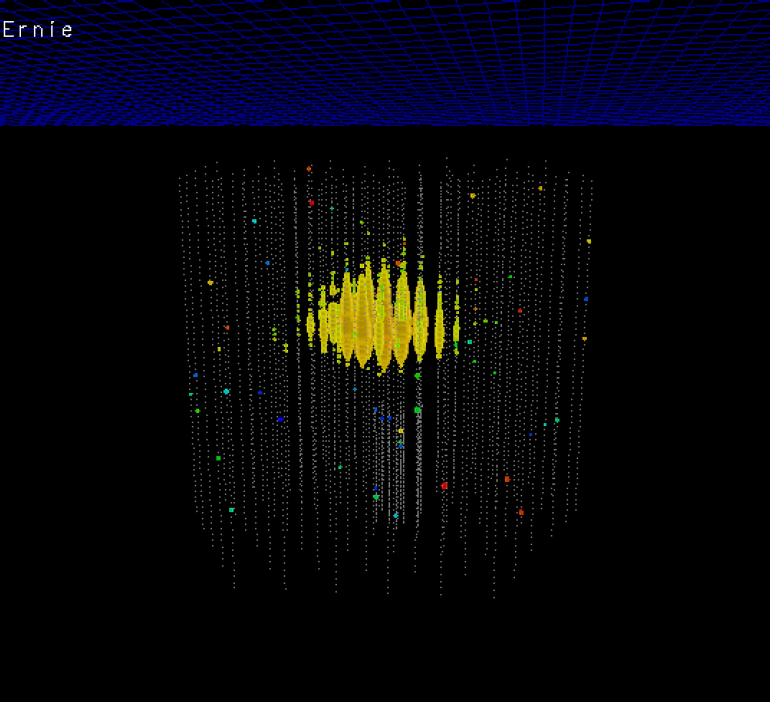
\includegraphics[keepaspectratio,width=13cm]{ernie}\\
$1.14 \pm 0.14$ PeV
\end{center}
{\blue P-value : $2.9 \cdot 10^{-3} \quad (2.8 \sigma)$}

\Tr
\onecolumn
\begin{center}
{\blue Try to get more "Muppets in the basket"}
\end{center}
%
\begin{itemize}
\item Perform a High-Energy Starting Event analysis (may 2010$-$may 2013)
\item[] Use event start veto criteria $\rightarrow$ remove atm. bkg $\mu$ and $\nu$ (showers)
\item[] Guarantees (contained) $\nu$ events and allows lower $E$ cut $\rightarrow 4\pi$
\end{itemize}
%
\begin{center}
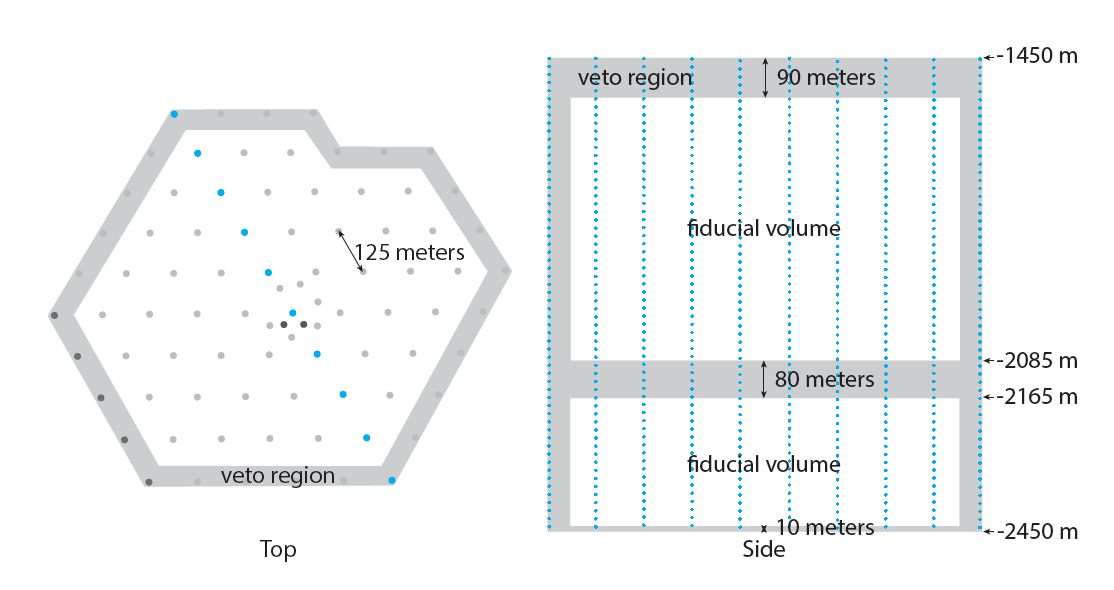
\includegraphics[keepaspectratio,height=10cm]{veto}
\end{center}

\Tr
\twocolumn[\begin{center}{\blue Several additional events were found}\end{center}]
%
\begin{center}
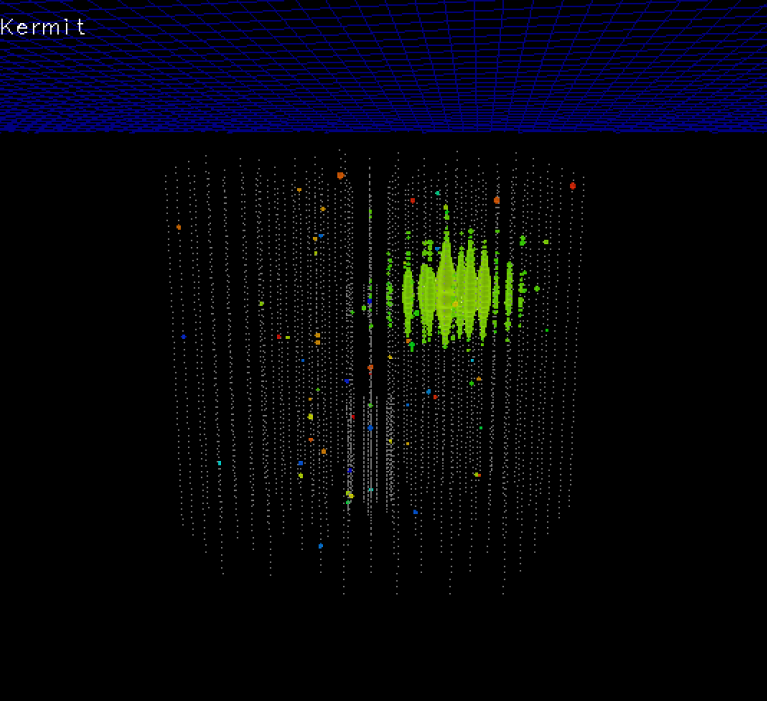
\includegraphics[keepaspectratio,width=13cm]{kermit}
\end{center}

\newpage

\begin{center}
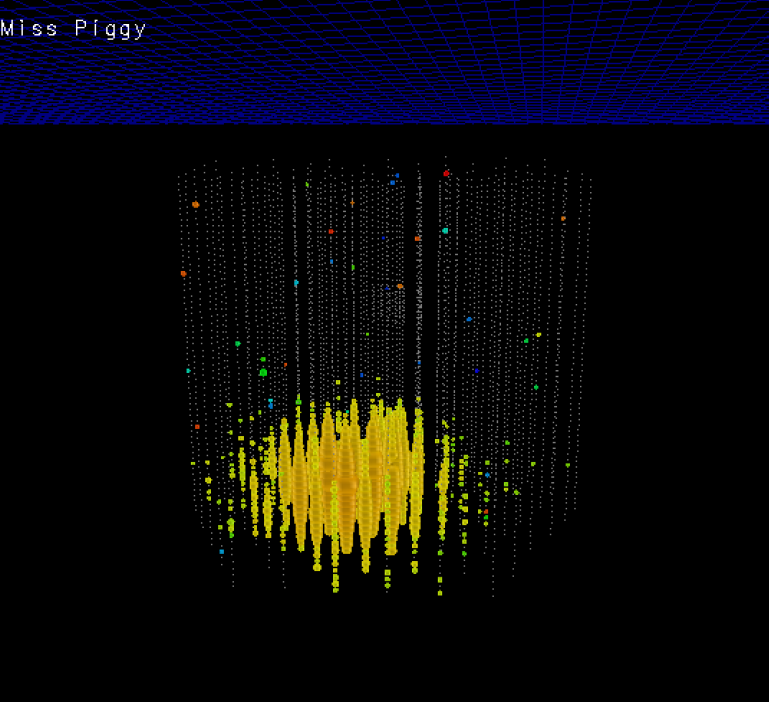
\includegraphics[keepaspectratio,width=13cm]{miss-piggy}
\end{center}

\Tr
\twocolumn[\begin{center}{\blue Also some $\mu$ track signatures}\end{center}]
%
\begin{center}
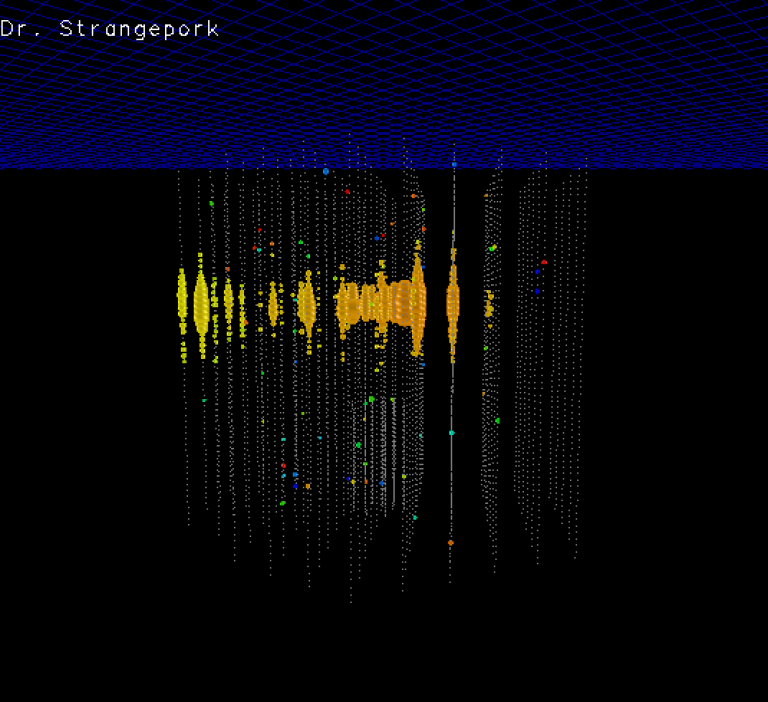
\includegraphics[keepaspectratio,width=13cm]{dr-strangepork}
\end{center}

\newpage

\begin{center}
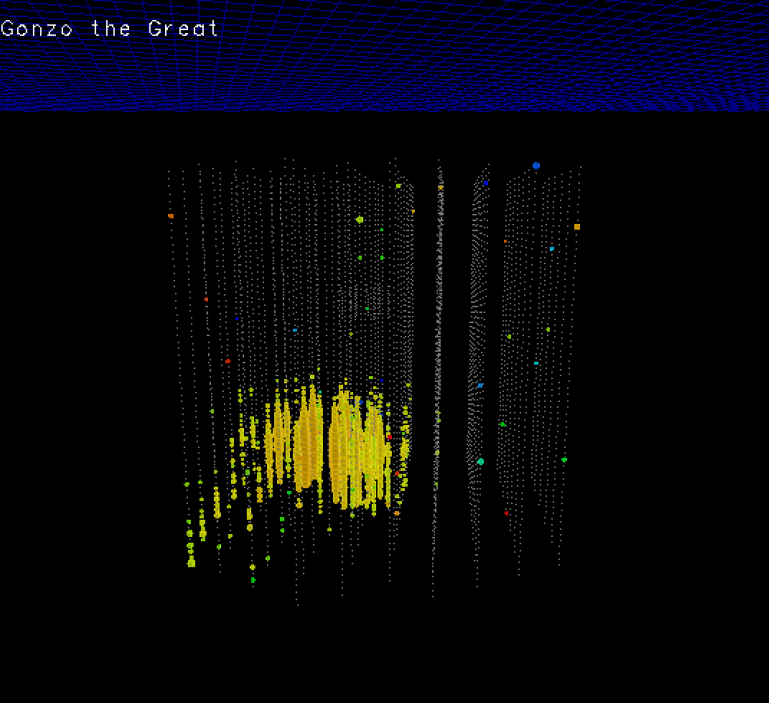
\includegraphics[keepaspectratio,width=13cm]{gonzo-the-great}
\end{center}

\Tr
\onecolumn
\begin{center}
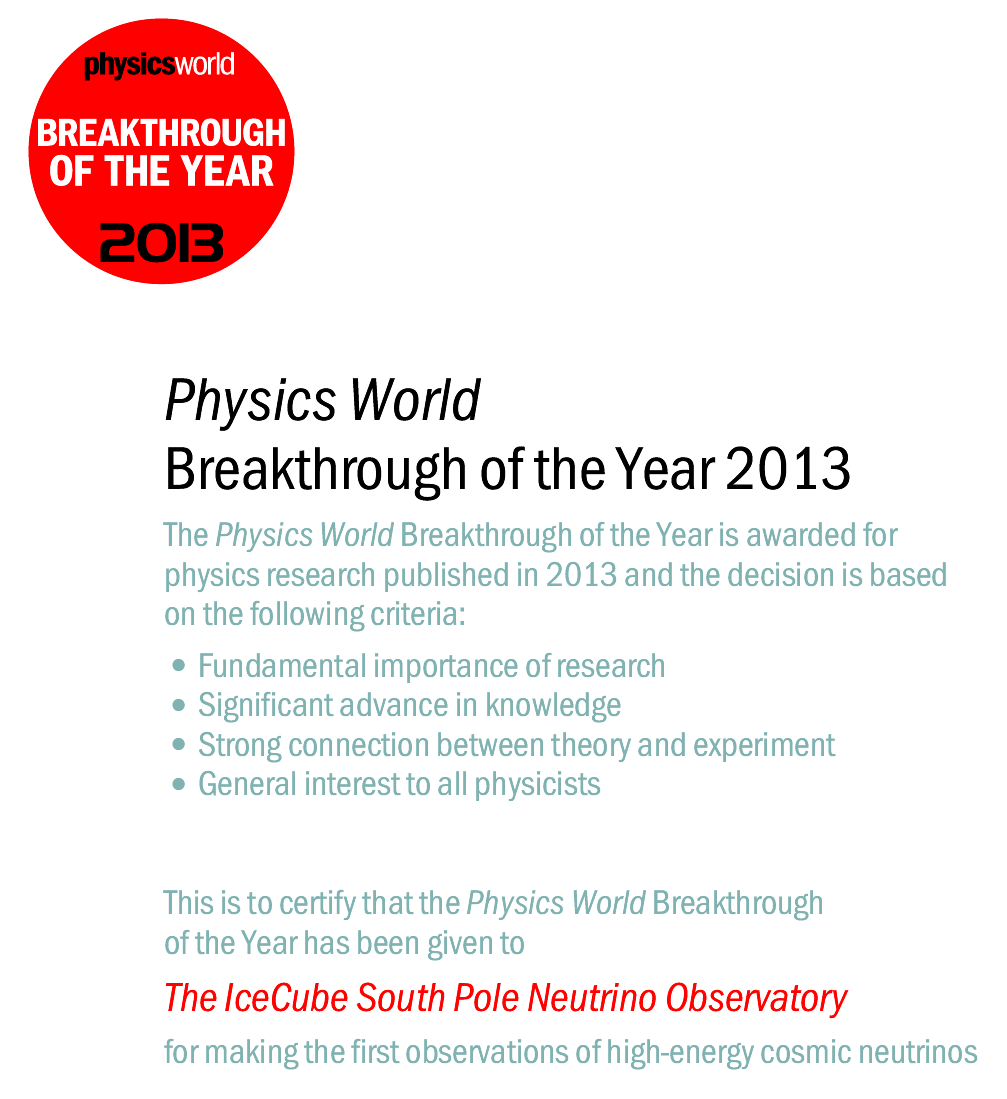
\includegraphics[keepaspectratio,height=15cm]{breakthrough}\\
\end{center}

\Tr
\onecolumn
\begin{center}
{\blue 82 observed Icecube High-Energy Starting Events (HESE)} {\large [C. Kopper, ICRC2017]}
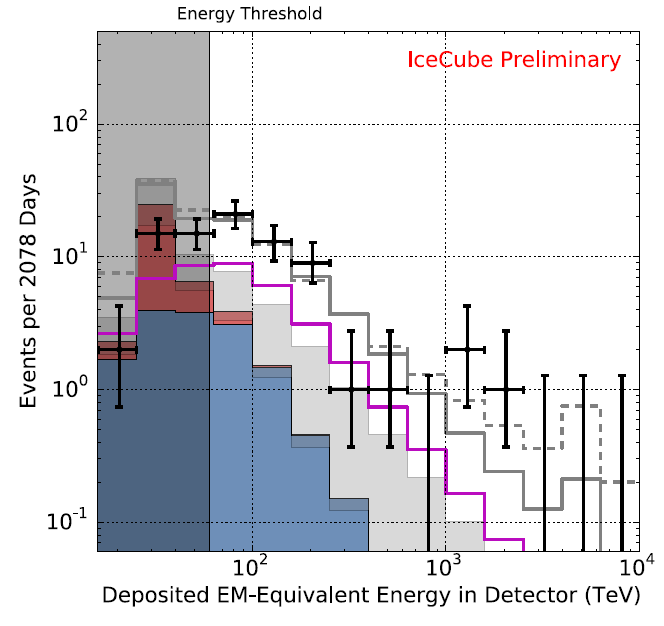
\includegraphics[keepaspectratio,height=11cm]{hese-e-6yr}
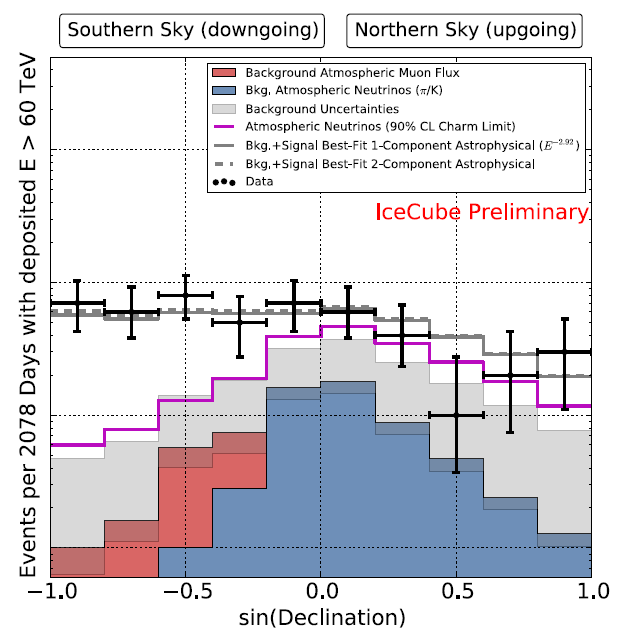
\includegraphics[keepaspectratio,height=11cm]{hese-decl-6yr}\\
\colorbox{yellow}{Evidence $(>7\sigma)$ for cosmic high-energy neutrinos}
\end{center}
What are the sources ?\\
Where are the multi-PeV events ?

\Tr
\onecolumn
\begin{center}
{\blue Source directions of the HESE events}\\[3mm]
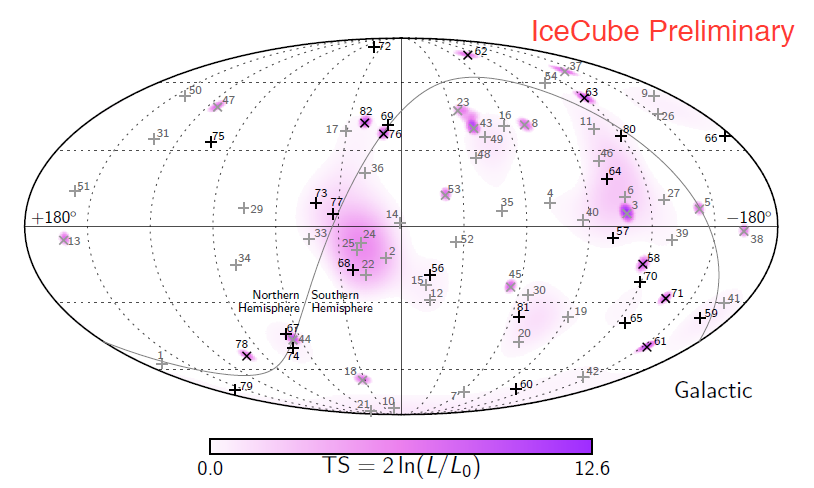
\includegraphics[keepaspectratio,height=13cm]{hese-skymap-gal-6yr}\\
\colorbox{yellow}{No evidence for point sources (yet)}
\end{center}

\Tr
\onecolumn
\begin{center}
{\blue IceCube observation (11-jun-2014) of a very energetic through-going muon}\\
$\alpha~:~$7h 21m 22s $\quad \delta~:~11.5^{\circ}$ {\large [ApJ 833 (2016) 3]}\\
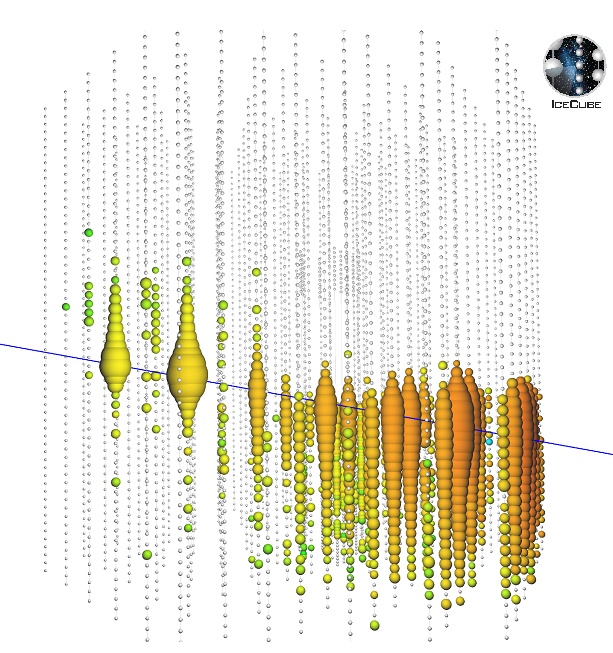
\includegraphics[keepaspectratio,height=13cm]{multi-pev-muon}\\
\colorbox{yellow}{Deposited energy $2.6 \pm 0.3~\rm{PeV} \rightarrow E_{\mu}=4-5~\rm{PeV} \rightarrow E_{\nu}>5~\rm{PeV}$}
\end{center}
